\chapter{Green's Functions}
In 1828, an English mathematician named George Green published "An Essay on the Application of Mathematical Analysis to the Theories of Electricity and Magnetism" with a theorem that is now used extensively to solve differential equations in electromagnetics, quantum mechanics, and applied mathematics \cite{green_phys_today}. Today, Green's functions are a useful tool in solving inhomogeneous differential equations and can be thought of as the impulse response for the differential equation. There are many excellent references for Green's functions from the mathematical perspective \cite{bender_orszag}, \cite{arfken_weber}, \cite{gbur_math}, \cite{guenther_partial_de}, \cite{duffy_green}, and for their application to electromagnetics \cite{jackson_classical_em}, \cite{zangwill_modern_em}, \cite{balanis_advanced}, \cite{goodman_fourier}, \cite{smith_radiation}.

\section{Time Dependence Sign Convention} \label{gf_sec:time_dependence}
Before getting started, we need to define the sign convention used for time dependence. We  assume harmonic propagating waves that follow the typical Engineering literature with time dependence going as $e^{j\omega t}$. This means we can represent a vector wave $\mathbf{A}(\mathbf{r},t)$ as:

\begin{equation}
\mathbf{A}\left(\mathbf{r},t\right) = \mathbf{A}\left(\mathbf{r}\right)e^{j\omega t}
\label{gf_eq:0a}
\end{equation}
\renewcommand{\baselinestretch}{2} \small\normalsize

\section{Green's Identities}
The two identities named for George Green will be derived here, starting from the divergence theorem:

\begin{equation}
\oint\limits_{S} \mathbf{A} \cdot \hat{n} dS = \int\limits_{V}d^3r'\nabla \cdot \mathbf{A}
\label{gf_eq:1}
\end{equation}
\renewcommand{\baselinestretch}{2} \small\normalsize

By replacing the vector $\mathbf{A}$ with a function of two arbitrary scalar variables, $\mathbf{A}=\varphi\nabla\psi$, we get:

\begin{equation}
\oint\limits_{S} \varphi\nabla\psi \cdot \hat{n} dS = \int\limits_{V}d^3r'\nabla \cdot \varphi\nabla\psi
\label{gf_eq:2}
\end{equation}
\renewcommand{\baselinestretch}{2} \small\normalsize

Using the identity $\nabla\psi\cdot \hat{n} = \frac{\partial \psi}{\partial n}$ and expanding the dot product in the volume integral yields Green's first identity:

\begin{equation}
\boxed{\oint\limits_{S} \varphi\frac{\partial \psi}{\partial n} dS = \int\limits_{V}d^3r' \left[ \nabla\varphi \cdot \nabla\psi +\varphi \nabla^2 \psi\right]}
\label{gf_eq:3}
\end{equation}
\renewcommand{\baselinestretch}{2} \small\normalsize

If we had flipped the order of the scalar variables and instead let $\mathbf{A}=\psi\nabla\varphi$, Green's first identity would be expressed as:
\begin{equation}
\oint\limits_{S} \psi\frac{\partial \varphi}{\partial n} dS = \int\limits_{V}d^3r' \left[ \nabla\psi \cdot \nabla\varphi +\psi \nabla^2 \varphi\right]
\label{gf_eq:4}
\end{equation}
\renewcommand{\baselinestretch}{2} \small\normalsize

\noindent Subtracting Equation \ref{gf_eq:4} from Equation \ref{gf_eq:3} yields Green's second identity:
\begin{equation}
\boxed{\oint\limits_{S} \left[ \varphi\frac{\partial \psi}{\partial n} - \psi\frac{\partial \varphi}{\partial n} \right]dS = \int\limits_{V}d^3r' \left[ \varphi\nabla^2\psi- \psi \nabla^2 \varphi\right]}
\label{gf_eq:5}
\end{equation}

\section{Method of Green's Functions}
We first consider scalar differential equations and outline how to obtain Green's functions in this case. For the purposes of this document, we are interested in time varying propagation problems. Therefore, we would like to apply the method of Green's functions to the scalar wave equation  to solve for the scalar field $\varphi$ as a function of space and time with an arbitrary driving function, $f$, that is also a function of space and time:

\begin{equation}
\nabla^2\varphi\left(\mathbf{r},t\right) - \frac{1}{c^2}\frac{\partial^2 \varphi\left(\mathbf{r},t\right)}{\partial t^2} = f\left(\mathbf{r},t\right)
\label{gf_eq:6}
\end{equation}
\renewcommand{\baselinestretch}{2} \small\normalsize

\noindent We can utilize the Fourier transform to remove the time dependence:

\begin{equation}
\nabla^2\varphi\left(\mathbf{r},\omega\right) + \frac{\omega^2}{c^2}\varphi\left(\mathbf{r},\omega\right) = f\left(\mathbf{r},\omega\right)
\label{gf_eq:7}
\end{equation}
\renewcommand{\baselinestretch}{2} \small\normalsize

Equation \ref{gf_eq:7} is the Helmholtz equation and it represents the wave equation with only spatial derivatives. If we use the wavevector, $k = \frac{\omega}{c}$, and suppress the variable dependence for clarity, Equation \ref{gf_eq:7} can be rewritten as:

\begin{equation}
\nabla^2\varphi + k^2\varphi = f
\label{gf_eq:8}
\end{equation}
\renewcommand{\baselinestretch}{2} \small\normalsize

The Green's function for this problem can be found by replacing the driving function, $f$, with a delta function:
\begin{equation}
\nabla^2G+ k^2G = -\delta\left(\mathbf{r}-\mathbf{r}' \right)
\label{gf_eq:9}
\end{equation}
\renewcommand{\baselinestretch}{2} \small\normalsize

Equation \ref{gf_eq:9} shows that the Green's function is the solution to the differential equation for a spatial impulse and therefore represents the impulse response of the system. The general method to find Green's functions is to solve the homogeneous differential equation (away from the delta function source) and then integrate over a small region that includes the delta function for normalization. Some authors, such as \cite{jackson_classical_em}, include a $4\pi$ scale factor with the delta function to absorb this normalization term into the differential equation rather than the Green's function.

Equations \ref{gf_eq:8} and \ref{gf_eq:9} can be rearranged to solve for the Laplacian, so that $\nabla^2\varphi = f - k^2\varphi$ and $\nabla^2G = -\delta\left(\mathbf{r}-\mathbf{r}' \right) - k^2G$. We can substitute these values into Green's second identity (Equation \ref{gf_eq:5}), with $\psi=G$:

\begin{equation}
\begin{gathered}
\oint\limits_{S} \left[ \varphi\frac{\partial G}{\partial n} - G\frac{\partial \varphi}{\partial n} \right]dS = \int\limits_{V}d^3r' \left[ \varphi\nabla^2G- G \nabla^2 \varphi\right] \\
\oint\limits_{S} \left[ \varphi\frac{\partial G}{\partial n} - G\frac{\partial \varphi}{\partial n} \right]dS = \int\limits_{V}d^3r' \left[ \varphi \left(-\delta\left(\mathbf{r}-\mathbf{r}' \right) - k^2G\right)- G \left(f - k^2\varphi \right)\right] \\
\int\limits_{V}d^3r'\varphi\delta\left(\mathbf{r}-\mathbf{r}' \right) = \oint\limits_{S}\left[G\frac{\partial \varphi}{\partial n} - \varphi\frac{\partial G}{\partial n} \right] +\int\limits_{V}d^3r'\left[ Gk^2\varphi - \varphi k^2G-k^2G - Gf \right] \\
\int\limits_{V}d^3r'\varphi\delta\left(\mathbf{r}-\mathbf{r}' \right) = \oint\limits_{S}\left[G\frac{\partial \varphi}{\partial n} - \varphi\frac{\partial G}{\partial n} \right] -\int\limits_{V}d^3r' Gf
\end{gathered}
\label{gf_eq:10}
\end{equation}
\renewcommand{\baselinestretch}{2} \small\normalsize

As long as $\mathbf{r}'$ is in the volume $V$, we can use the sifting property of the delta function to provide an explicit representation for $\varphi$:
\begin{equation}
\boxed{\varphi = \oint\limits_{S}\left[G\frac{\partial \varphi}{\partial n} - \varphi\frac{\partial G}{\partial n} \right] -\int\limits_{V}d^3r' Gf}
\label{gf_eq:11}
\end{equation}
\renewcommand{\baselinestretch}{2} \small\normalsize

\section{Boundary Conditions}
There are two traditional types of boundary conditions: Dirichlet, where $\varphi$ is specified on the boundary, or Neuman, where the normal derivative of $\varphi$ is specified on the boundary. There is a third type of boundary condition, known as the Robin condition, that is a weighted combination of Dirichlet and Neuman boundary conditions.

\subsection{Dirichlet Boundary Conditions}
For Dirichlet boundary conditions, the solution is specified on the surface, $\varphi\left(\mathbf{r}\right) |_{S} = \varphi\left(\mathbf{r}_S \right) = a\left(\mathbf{r}_s\right)$. To simplify Equation \ref{gf_eq:11}, we can enforce the following condition on the Green's function:

\begin{equation}
G\left(\mathbf{r},\mathbf{r}' \right)\bigg|_{S}=0
\label{gf_eq:12}
\end{equation}
\renewcommand{\baselinestretch}{2} \small\normalsize

Green's functions specified in this manner are often called Green's functions of the first kind. Substituting Equation \ref{gf_eq:12} into Equation \ref{gf_eq:11} results in the following equation for $\varphi$:
\begin{equation}
\boxed{\varphi = -\oint\limits_{S} \varphi\frac{\partial G}{\partial n} -\int\limits_{V}d^3r' Gf}
\label{gf_eq:13}
\end{equation}
\renewcommand{\baselinestretch}{2} \small\normalsize

\subsection{Neuman Boundary Conditions}
For Neuman boundary conditions, the normal derivative of the field is specified on the surface, $\frac{\partial\varphi\left(\mathbf{r}\right)}{\partial n}|_{S} = b\left(\mathbf{r}_s\right)$. As described in \cite{jackson_classical_em}, \cite{zangwill_modern_em}, and \cite{balanis_advanced}, we cannot simply set the normal derivative of $G$ to $0$. This can be demonstrated by integrating Equation \ref{gf_eq:9} over a volume and then applying the divergence theorem:

\begin{equation}
\begin{gathered}
\int\limits_{V}d^3r' \nabla^2 G = \int\limits_{V}d^3r'\left[-\delta\left(\mathbf{r}-\mathbf{r}' \right) -k^2G \right] \\
\int\limits_{V}d^3r' \nabla \cdot \nabla G = -\int\limits_{V}d^3r'\delta\left(\mathbf{r}-\mathbf{r}' \right) -\int\limits_{V}d^3r'k^2G \\
\oint\limits_{S}\nabla G \cdot \hat{n} dS  = -1 - \int\limits_{V}d^3r'k^2G\\
\oint\limits_{S}\frac{\partial G}{\partial n} dS = -1 - \int\limits_{V}d^3r' k^2G
\end{gathered}
\label{gf_eq:14}
\end{equation}
\renewcommand{\baselinestretch}{2} \small\normalsize

Equation \ref{gf_eq:14} must hold for all values of $k$, so we can find a general condition for $\frac{\partial G}{\partial n}$ by letting $k = 0$:

\begin{equation}
\oint\limits_{S}\frac{\partial G}{\partial n} dS = -1
\label{gf_eq:15}
\end{equation}
\renewcommand{\baselinestretch}{2} \small\normalsize

Equation \ref{gf_eq:15} indicates that there is a discontinuity in the normal derivative of the Green's function. Letting $S$ be the total surface area gives us the following condition on the normal derivative of the Green's function:
\begin{equation}
\frac{\partial G}{\partial n} = -\frac{1}{S}
\label{gf_eq:16}
\end{equation}
\renewcommand{\baselinestretch}{2} \small\normalsize

Equation \ref{gf_eq:16} demonstrates the jump condition for the normal derivative of the Green's function. Note that when the surface is taken out to infinity that $\frac{\partial G}{\partial n} = 0$. Green's functions specified in this manner are often called Green's functions of the second kind. Substituting Equation \ref{gf_eq:16} into Equation \ref{gf_eq:11} results in the following equation for $\varphi$:

\begin{equation}
\boxed{\varphi = \oint\limits_{S}\left[G\frac{\partial \varphi}{\partial n} + \frac{\varphi}{S} \right] -\int\limits_{V}d^3r' Gf}
\label{gf_eq:17}
\end{equation}
\renewcommand{\baselinestretch}{2} \small\normalsize

We can rewrite Equation \ref{gf_eq:17} as in \cite{jackson_classical_em}, using the average value of the solution over the surface, $\left< \varphi\right> = \frac{1}{S}\oint\limits_{S}\varphi dS$:
\begin{equation}
\boxed{\varphi = \left<\varphi \right> + \oint\limits_{S}G\frac{\partial \varphi}{\partial n}  -\int\limits_{V}d^3r' Gf}
\label{gf_eq:18}
\end{equation}
\renewcommand{\baselinestretch}{2} \small\normalsize

\subsection{Robin Boundary Conditions}

\section{Properties of Green's Functions} \label{gf_sec:properties}
We have already discussed the fact that Green's functions represent the spatial impulse response of the differential equation. This section introduces some other properties of Green's functions, including causality, reciprocity, continuity, and general forms.

\subsection{Causality} \label{gf_sec:causality}
For a system to be causal, it may only depend on past or present inputs and not on future inputs. Any physically realizable system, such as an electromagnetic wave must be causal, as something that has not yet happened cannot have an impact on the current output. We can relate the causality condition through the phase with the restriction that the phase can be delayed but not advanced. This tells us that for propagating waves, we need to look for solutions in the form of $g\left(\pm\left[\omega t - kr\right]\right)$, as solutions in the form of $g\left(\pm\left[\omega t + kr\right]\right)$ advance the phase and are not physically realizable. With the time dependence as specified in Section \ref{gf_sec:time_dependence}, our solutions must have the following form:

\begin{equation}
G\left(r,t\right) \sim g\left(\omega t - kr\right)
\label{gf_eq:18a}
\end{equation}
\renewcommand{\baselinestretch}{2} \small\normalsize

Equation \ref{gf_eq:18a} tells us that for physically realizable propagating waves, the signs of $\omega t$ and $kr$ must be different. We can also think of $g\left(\omega t - kr\right)$ as representing an outward traveling wave from the origin and $g\left(\omega t + kr\right)$ as representing an inward propagating wave from $\infty$. With this restriction, our vector waves from Equation \ref{gf_eq:0a} must take the form:

\begin{equation}
\mathbf{A}\left(\mathbf{r},t\right) = \mathbf{A}e^{j\left(\omega t - \mathbf{k} \cdot \mathbf{r} \right)}
\label{gf_eq:18b}
\end{equation}
\renewcommand{\baselinestretch}{2} \small\normalsize

Since the Green's functions represent the impulse response, they will have the same spatial dependence as Equation \ref{gf_eq:18b}.

\subsection{Reciprocity} \label{gf_sec:reciprocity}
Green's functions must be symmetric with respect to $\mathbf{r}$ (the vector to the observer) and $\mathbf{r}'$ (the vector to the source), so that:

\begin{equation}
G\left(\mathbf{r},\mathbf{r}' \right) = G\left(\mathbf{r}',\mathbf{r} \right)
\label{gf_eq:18c}
\end{equation}
\renewcommand{\baselinestretch}{2} \small\normalsize

This property is known as reciprocity and it tells us that the impulse reponse for a propagating wave is the same in both directions. Reciprocity is commonly used in antenna radiation analysis as it allows us to analyze an antenna considering it as either a transmitter or a receiver.

\subsection{Continuity} \label{gf_sec:continuity}
A necessary condition for reciprocity is that Green's functions must be continuous in all space except $\mathbf{r} = \mathbf{r}'$.

\subsection{General Forms}
Because Green's functions are the spatial impulse response of the system, we can expect them to be used in a convolution integral. With that in mind, Green's functions usually take the form:
\begin{equation}
G\left(\mathbf{r},\mathbf{r}' \right) = g\left( \mathbf{r} - \mathbf{r}'\right)
\label{gf_eq:18d}
\end{equation}
\renewcommand{\baselinestretch}{2} \small\normalsize

Using the results of the previously described properties, the most general representation of a Green's function is as follows:

\begin{equation}
G\left(\mathbf{r},\mathbf{r}',t \right) = g\left(\omega t - k| \mathbf{r} - \mathbf{r}' | \right)
\label{gf_eq:19b}
\end{equation}
\renewcommand{\baselinestretch}{2} \small\normalsize

\section{Free Space Green's Functions}
This section demonstrates solving for the free space Green's functions for the Helmholtz equation (Equation \ref{gf_eq:9}) in both 3-dimensions and 2-dimensions. In free space, there are no boundaries, so we can let $r\rightarrow \infty$ and use Dirichlet boundary conditions. Without loss of generality, we can place the delta function at the origin, so that $\delta\left(\mathbf{r}-\mathbf{r}' \right) \rightarrow \delta \left(\mathbf{r} \right)$. To find the Green's function, we need to solve the homogeneous equation away from the delta function and then integrate over a small region around the origin for normalization. The homogenous equation to solve is:

\begin{equation}
\nabla^2G+ k^2G = 0
\label{gf_eq:19}
\end{equation}
\renewcommand{\baselinestretch}{2} \small\normalsize

Because the delta function is rotationally symmetric, the Green's function must also be rotationally symmetric.

\subsection{3-Dimensions}\label{gf_sec:3d}
This section derives the free space Green's function for the Helmholtz equation in 3-dimensional space. Because we used the Fourier transform to remove the time dependence from the wave equation (Equation 
\ref{gf_eq:6}), we will first work in the frequency domain and then transform the result back to the time domain.

\subsubsection{Deriviation in the Frequency Domain}
In 3-dimensions,  rotational symmetry means that  $\frac{\partial G}{\partial\theta} = \frac{\partial G}{\partial\phi}=0$. Therefore we can expand the Laplacian of Equation \ref{gf_eq:19} in spherical coordinates and neglect the $\theta$ and $\phi$ components:

\begin{equation}
\frac{1}{r^2}\frac{\partial}{\partial r}\left(r^2\frac{\partial G}{\partial r}\right)+ k^2G = 0
\label{gf_eq:20}
\end{equation}
\renewcommand{\baselinestretch}{2} \small\normalsize

Expanding the derivatives in Equation \ref{gf_eq:20} along with a little algebraic manipulation allows us to rewrite this into something more manageable:
\begin{equation}
\begin{gathered}
\frac{1}{r^2}\left[2r\frac{\partial G}{\partial r}+ r^2\frac{\partial^2 G}{\partial r^2}  \right] + k^2G = 0 \\
r\frac{\partial^2 G}{\partial r^2} + 2\frac{\partial G}{\partial r}+ k^2rG = 0 \\
\frac{\partial^2 \left(rG\right)}{\partial r^2} + k^2rG = 0
\end{gathered}
\label{gf_eq:21}
\end{equation}
\renewcommand{\baselinestretch}{2} \small\normalsize

Equation \ref{gf_eq:21} has the following  solution:

\begin{equation}
G = c_1\frac{e^{jkr}}{r} + c_2\frac{e^{-jkr}}{r}
\label{gf_eq:22}
\end{equation}
\renewcommand{\baselinestretch}{2} \small\normalsize

From the causality restriction discussed in Section \ref{gf_sec:causality}, the $c_2$ term describes an outward propagating wave. This is the physical solution, which means $c_1$ must be equal to $0$. Therefore, the free space Green's function is:

\begin{equation}
G = c_2\frac{e^{-jkr}}{r}
\label{gf_eq:23}
\end{equation}
\renewcommand{\baselinestretch}{2} \small\normalsize

This equation is valid everywhere except $r=0$. To find $c_2$, we need to integrate Equation \ref{gf_eq:9} over a small volume centered at $r=0$ and then take the limit as $r\rightarrow0$.

\begin{equation}
\begin{gathered}
\lim_{r\to0}\int\limits_{V}d^3r'\left[\nabla^2G+ k^2G\right] = -\lim_{r\to0}\int\limits_{V}\delta\left(\mathbf{r}\right) \\
\lim_{r\to0}\int\limits_{V}d^3r'\left[\nabla \cdot\nabla G+ k^2G\right] = -1 \\
\lim_{r\to0}\left[\oint\limits_{S}\nabla G \cdot \hat{n} dS + \int\limits_{V}d^3r' k^2G\right] = -1 \\
\lim_{r\to0}\left[\oint\limits_{S}\frac{\partial G}{\partial n} dS + \int\limits_{V}d^3r' k^2G\right] = -1
\end{gathered}
\label{gf_eq:24}
\end{equation}
\renewcommand{\baselinestretch}{2} \small\normalsize

Substituting Equation \ref{gf_eq:23} in for $G$ and letting $\hat{n} = \hat{r}$, $dS = r'^2\sin{\theta'}d\theta' d\phi'$, and  $d^3r' = r'^2\sin{\theta'}dr'd\theta' d\phi'$ yields:

\begin{equation}
\begin{gathered}
\lim_{r\to0}\left[c_2\oint\limits_{S}\frac{\partial }{\partial r'}\frac{e^{-jkr'}}{r'} r'^2\sin{\theta'} d\theta' d\phi '+ c_2\int\limits_{V}r'^2 \sin{\theta'}dr' d\theta' d\phi' k^2\frac{e^{-jkr'}}{r'}\right] = -1 \\
\lim_{r\to0}\left[c_2 r^2\left( \frac{jk}{r} - \frac{1}{r^2}\right)e^{-jkr}\oint\limits_{S}\sin{\theta'} d\theta' d\phi' + c_2\int\limits_{V}dr' d\theta' d\phi' k^2r'e^{-jkr'}\sin{\theta'}\right] = -1 \\
\lim_{r\to0}\left[4\pi c_2 \left( jkr - 1\right)e^{-jkr}+ 4\pi c_2k^2\int\limits_{V}dr' r'e^{-jkr'}\right] = -1 \\
\lim_{r\to0}4\pi c_2\left[\left( jkr - 1\right)e^{-jkr}+ k^2\int\limits_{V}dr' \frac{\partial}{\partial k}\frac{e^{-jkr'}}{j}\right] = -1 \\
4\pi c_2\left[-1 +  \lim_{r\to0}\frac{k^2}{j}\frac{\partial}{\partial k}\left( \frac{-1}{jk}e^{-jkr'}\right)\bigg|_0^{r}  \right] = -1 \\
-4\pi c_2\left[1 - \lim_{r\to0}k^2\frac{\partial}{\partial k}\left( \frac{1}{k}e^{-jkr} - \frac{1}{k}\right) \right] = -1 \\
c_2\left[1 - \lim_{r\to0}k^2\left(-\frac{1}{k^2}+\frac{-jre^{-jkr}}{k}+\frac{1}{k^2}\right) \right] = \frac{1}{4\pi} \\
 c_2 = \frac{1}{4\pi}
\end{gathered}
\label{gf_eq:25}
\end{equation}
\renewcommand{\baselinestretch}{2} \small\normalsize

Now letting $r \rightarrow |\mathbf{r}-\mathbf{r}'|$, we have the final free space 3-dimensional Green's function, $G_o$:

\begin{equation}
\boxed{G_o\left(\mathbf{r},\mathbf{r}'\right) = \frac{e^{-jk|\mathbf{r} - \mathbf{r}'|}}{4\pi |\mathbf{r} - \mathbf{r}'|}}
\label{gf_eq:26}
\end{equation}
\renewcommand{\baselinestretch}{2} \small\normalsize

As discussed for Equation \ref{gf_eq:9}, some authors, such as \cite{jackson_classical_em}, include the $4\pi$ scale factor with the delta function. In this case, the free space 3-dimensional Green's function is:
\begin{equation}
G_o\left(\mathbf{r},\mathbf{r}'\right)  = \frac{e^{-jk|\mathbf{r} - \mathbf{r}'|}}{|\mathbf{r} - \mathbf{r}'|}
\label{gf_eq:27}
\end{equation}
\renewcommand{\baselinestretch}{2} \small\normalsize

To help visualize this Green's function, the magnitude and phase is shown in Figure \ref{gf_fig:1} and the real and imaginary components are shown in Figure \ref{gf_fig:2}. These figures constrain the Green's function to the $x-y$ plane for visualization.

\begin{figure}[H]
\begin{center}
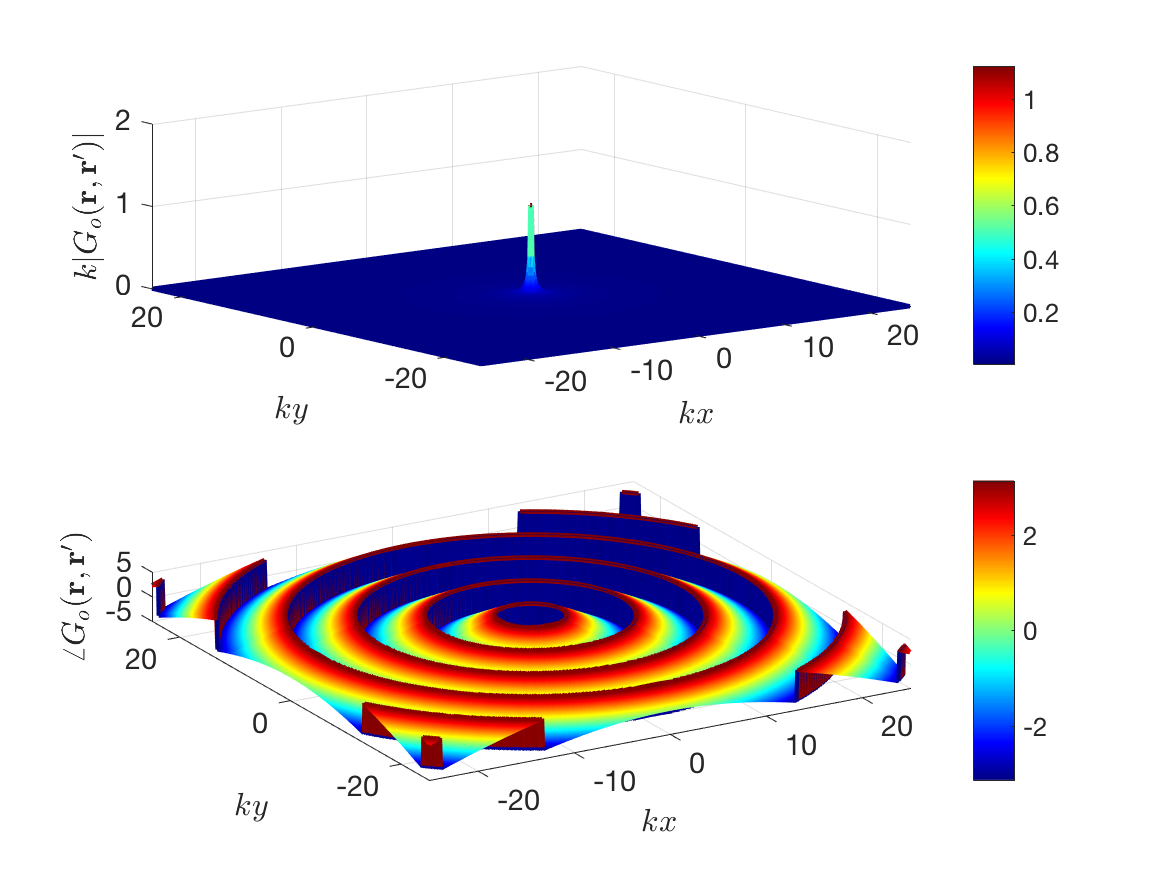
\includegraphics[width=3in]{../media/3d_fs_gf_mag.png}
\end{center}
\renewcommand{\baselinestretch}{1}
\small\normalsize
\begin{quote}
\caption[Magnitude and Phase of 3-D Free Space Green's Function]{ Magnitude and Phase of 3-D Free Space Green's Function\label{gf_fig:1}}
\end{quote}
\end{figure} 
\renewcommand{\baselinestretch}{2}
\small\normalsize

\begin{figure}[H]
\begin{center}
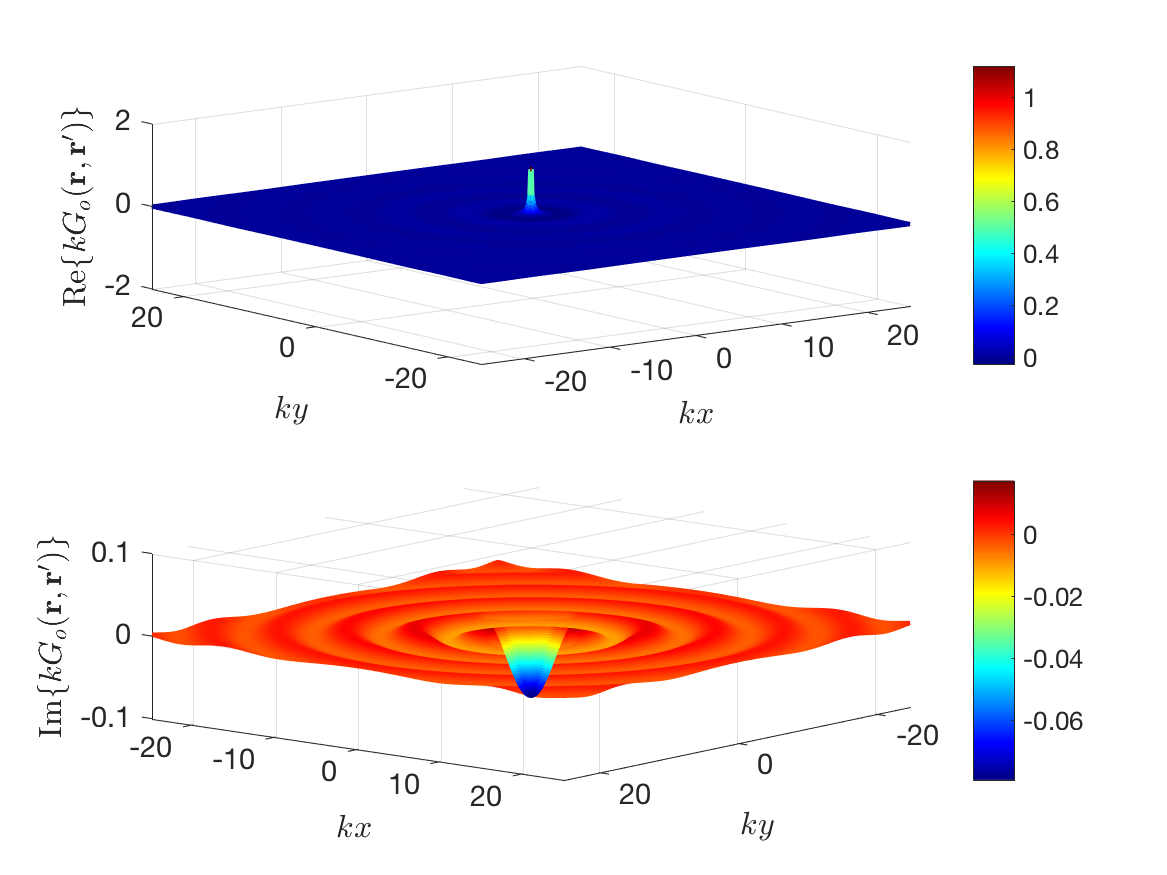
\includegraphics[width=3in]{../media/3d_fs_gf_re_im.png}
\end{center}
\renewcommand{\baselinestretch}{1}
\small\normalsize
\begin{quote}
\caption[Real and Imaginary Components of 3-D Free Space Green's Function]{Real and Imaginary Components of 3-D Free Space Green's Function \label{gf_fig:2}}
\end{quote}
\end{figure} 
\renewcommand{\baselinestretch}{2}
\small\normalsize

\subsubsection{Conversion to the Time Domain}
The Green's function in Equation \ref{gf_eq:26} is still in Fourier space. We can clearly express the frequency dependence as:

\begin{equation}
G_o\left(\mathbf{r},\mathbf{r}',\omega\right) = \frac{e^{-j\frac{\omega}{c}|\mathbf{r} - \mathbf{r}'|}}{4\pi |\mathbf{r} - \mathbf{r}'|}
\label{gf_eq:28}
\end{equation}
\renewcommand{\baselinestretch}{2} \small\normalsize

To determine the Green's function in the time domain, we need to take the inverse Fourier transform:
\begin{equation}
\begin{gathered}
G_o\left(\mathbf{r},\mathbf{r}',t\right) = \frac{1}{2\pi}\int\limits_{-\infty}^{\infty}d\omega e^{-j\omega t}G_o\left(\mathbf{r},\mathbf{r}',\omega\right) \\
G_o\left(\mathbf{r},\mathbf{r}',t\right) = \frac{1}{2\pi}\int\limits_{-\infty}^{\infty}d\omega e^{-j\omega t}  \frac{e^{-j\frac{\omega}{c}|\mathbf{r}-\mathbf{r}'|}}{4\pi |\mathbf{r}-\mathbf{r}'|}\\
G_o\left(\mathbf{r},\mathbf{r}',t\right) = \frac{1}{4\pi |\mathbf{r}-\mathbf{r}'|}\frac{1}{2\pi}\int\limits_{-\infty}^{\infty}d\omega e^{-j\omega\left(t- \frac{|\mathbf{r}-\mathbf{r}'|}{c}\right)}
\end{gathered}
\label{gf_eq:29}
\end{equation}
\renewcommand{\baselinestretch}{2} \small\normalsize

Recognizing that the Fourier transform of the delta function is:
\begin{equation}
\delta(t-t_0) = \frac{1}{2\pi}\int\limits_{-\infty}^{\infty}d\omega e^{-j\omega \left(t-t_0\right)}
\label{gf_eq:30}
\end{equation}
\renewcommand{\baselinestretch}{2} \small\normalsize

We can write the free space Green's function in the temporal domain as:
\begin{equation}
\boxed{G_o\left(\mathbf{r},\mathbf{r}',t\right) = \frac{\delta\left(t-\frac{|\mathbf{r}-\mathbf{r}'|}{c} \right)}{4\pi |\mathbf{r}-\mathbf{r}'|}}
\label{gf_eq:31}
\end{equation}
\renewcommand{\baselinestretch}{2} \small\normalsize

Equation \ref{gf_eq:31} assumes the source is turned on at time $0$. If we let the source be turned on at an arbitrary time, $t'$, a more general expression is:
\begin{equation}
G_o\left(\mathbf{r},\mathbf{r}',t,t'\right) = \frac{\delta\left(t-t'-\frac{|\mathbf{r}-\mathbf{r}'|}{c} \right)}{4\pi |\mathbf{r}-\mathbf{r}'|}
\label{gf_eq:32}
\end{equation}
\renewcommand{\baselinestretch}{2} \small\normalsize

In the time domain, we generally refer to $G_o\left(\mathbf{r},\mathbf{r}',t\right)$ as the retarded wave solution because an observer will experience the source as if it acted at an earlier (retarded) time, $t_1=t-t'-\frac{|\mathbf{r}-\mathbf{r}'|}{c}$.

\subsubsection{Example of Use}
The 3-dimensional free space Green's function is extremely useful in scalar diffraction theory and Fourier optics \cite{goodman_fourier}, \cite{born_wolf_po}.

\subsection{2-Dimensions}\label{gf_sec:2d}
This section derives the free space Green's function for the Helmholtz equation in 2-dimensional space. Because we used the Fourier transform to remove the time dependence from the wave equation (Equation \ref{gf_eq:6}), we will first work in the frequency domain and then transform the result back to the time domain.

\subsubsection{Deriviation in the Frequency Domain}
In 2-dimensions,  rotational symmetry means that  $\frac{\partial G}{\partial\phi} =0$. Therefore we can expand the Laplacian of Equation \ref{gf_eq:19} in polar coordinates and neglect the $\phi$ components:

\begin{equation}
\frac{1}{\rho}\frac{\partial}{\partial \rho}\left(\rho\frac{\partial G}{\partial \rho}\right)+ k^2G = 0
\label{gf_eq:33}
\end{equation}
\renewcommand{\baselinestretch}{2} \small\normalsize

\noindent Equation \ref{gf_eq:33} is Bessel's equation with $\nu = 0$:
\begin{equation}
\frac{1}{\rho}\frac{\partial}{\partial \rho}\left(\rho\frac{\partial G}{\partial \rho}\right)+ \left(k^2 -\nu^2\right)G = 0
\label{gf_eq:34}
\end{equation}
\renewcommand{\baselinestretch}{2} \small\normalsize

\noindent The general solution to Equation \ref{gf_eq:33} is 
\begin{equation}
G = c_1J_0\left(k\rho\right) + c_2N_0\left(k\rho\right)
\label{gf_eq:35}
\end{equation}
\renewcommand{\baselinestretch}{2} \small\normalsize

Here $J_0$ is a Bessel function of the first kind, and $N_0$ is a Bessel function of the second kind. Since the delta function is singular at the origin, we cannot demand that $G$ be finite at the origin. This means that $c_2 \neq 0$ and we have one equation with two unknowns.

When working with propagating waves, it is sometimes more useful to work with Hankel functions than Bessel functions. The Hankel functions are:
\begin{equation}
\begin{gathered}
H_0^{(1)}(k\rho) = J_0(k\rho) + jN_0(k\rho) \\
H_0^{(2)}(k\rho) = J_0(k\rho) - jN_0(k\rho)
\label{gf_eq:36}
\end{gathered}
\end{equation}
\renewcommand{\baselinestretch}{2} \small\normalsize

The Hankel functions behave asymptotically like waves as can be seen by their behavior for large arguments \cite{abramowitz_stegun}, which can be derived from the integral representation through the saddle point method \cite{arfken_weber}:
\begin{equation}
\begin{gathered}
H_0^{(1)}(k\rho) \approx \sqrt{\frac{2}{\pi k\rho}}e^{j\left(k\rho - \frac{\pi}{4}\right)}\\
H_0^{(2)}(k\rho) \approx \sqrt{\frac{2}{\pi k\rho}}e^{-j\left(k\rho - \frac{\pi}{4}\right)}
\label{gf_eq:36a}
\end{gathered}
\end{equation}
\renewcommand{\baselinestretch}{2} \small\normalsize

We can now represent the solution to Equation \ref{gf_eq:33} in terms of Hankel functions as:
\begin{equation}
G = c_1H_0^{(1)}\left(k\rho\right) +c_2H_0^{(2)}\left(k\rho\right) 
\label{gf_eq:37}
\end{equation}
\renewcommand{\baselinestretch}{2} \small\normalsize

From the causality discussion in Section \ref{gf_sec:causality}, $H_0^{(2)}$ acts like an outward propagating wave while $H_0^{(1)}$ acts like an inward propagating wave. Therefore, $H_0^{(2)}$ is the physical solution, $c_1=0$, and the Green's function is:

\begin{equation}
G = c_2H_0^{(2)}\left(k\rho\right) 
\label{gf_eq:38}
\end{equation}
\renewcommand{\baselinestretch}{2} \small\normalsize

As in Section \ref{gf_sec:3d}, we integrate Equation \ref{gf_eq:9} over a small disk, $D$, centered at $\rho = 0$ and take the limit as $\rho \rightarrow 0$. For small arguments, the asymptotic behavior of $H_0^{(2)}(k\rho) \sim -j\frac{2}{\pi}\ln\left({k\rho}\right)$ and we can substitute $G = -\frac{j2c_1}{\pi}\ln\left({k\rho}\right)$ \cite{abramowitz_stegun}. 

\begin{equation}
\begin{gathered}
\lim_{\rho\to 0}\int\limits_{D} \left[ \frac{1}{\rho'}\frac{\partial}{\partial \rho'}\left(\rho' \frac{\partial G}{\partial \rho'} \right) + k^2G\right]\rho' d\rho' d\theta' = \lim_{\rho\to 0}\int\limits_{D} \delta\left(\boldsymbol{\rho}-\boldsymbol{\rho}' \right)\rho' d\rho' d\phi' \\
\lim_{\rho\to 0}\int\limits_{D} \left[ -\frac{1}{\rho'}\frac{\partial}{\partial \rho'}\left(\rho' jc_1\frac{2}{\pi}\frac{\partial \ln(k\rho')}{\partial \rho'} \right) - k^2jc_1\frac{2}{\pi}\ln(k\rho')\right]\rho' d\rho' d\theta' = -1 \\
\lim_{\rho\to 0}-4jc_1\int\limits_{D} \left[\frac{\partial}{\partial \rho'}\left(\rho' \frac{\partial \ln(k\rho')}{\partial \rho'} \right) + k^2\rho'\ln(k\rho')\right] d\rho' = -1 \\
\lim_{\rho\to 0}4jc_1\left[\left(\rho' \frac{1 }{\rho'} \right)\bigg|_0^{\rho} + \int\limits_{D}k^2\rho'\ln(k\rho') d\rho'\right] = 1 \\
\lim_{\rho\to 0}c_1\left[ 1 +  k^2\left( \ln(k\rho')\frac{\rho'^2}{2}\bigg|_0^{\rho} - \int\limits_{D}\frac{\rho'^2}{2}\frac{1}{\rho'} d\rho' \right)\right] = -\frac{j}{4} \\
\lim_{\rho\to 0}c_1\left[ 1 +  k^2\left( \ln(k\rho)\frac{\rho^2}{2} - \frac{1}{2}\int\limits_{D}\rho' d\rho' \right)\right] = -\frac{j}{4} \\
\lim_{\rho\to 0}c_1\left[ 1 - \frac{\rho^2}{4}\right] = \frac{j}{4} \\
c_1 = -\frac{j}{4}
\end{gathered}
\label{gf_eq:39}
\end{equation}
\renewcommand{\baselinestretch}{2} \small\normalsize

Now letting $\rho \rightarrow |\boldsymbol{\rho}-\boldsymbol{\rho}'|$, we have the final free space 2-dimensional Green's function, $G_o$:

\begin{equation}
\boxed{G_o\left(\boldsymbol{\rho},\boldsymbol{\rho}'\right) = -\frac{j}{4}H_0^{(2)}\left(k|\boldsymbol{\rho} - \boldsymbol{\rho}' | \right)}
\label{gf_eq:40}
\end{equation}
\renewcommand{\baselinestretch}{2} \small\normalsize

To help visualize this Green's function, the magnitude and phase is shown in Figure \ref{gf_fig:3} and the real and imaginary components are shown in Figure \ref{gf_fig:4}. The real and imaginary components show the sinusoidal behavior of the Hankel functions for large arguments.

\begin{figure}[H]
\begin{center}
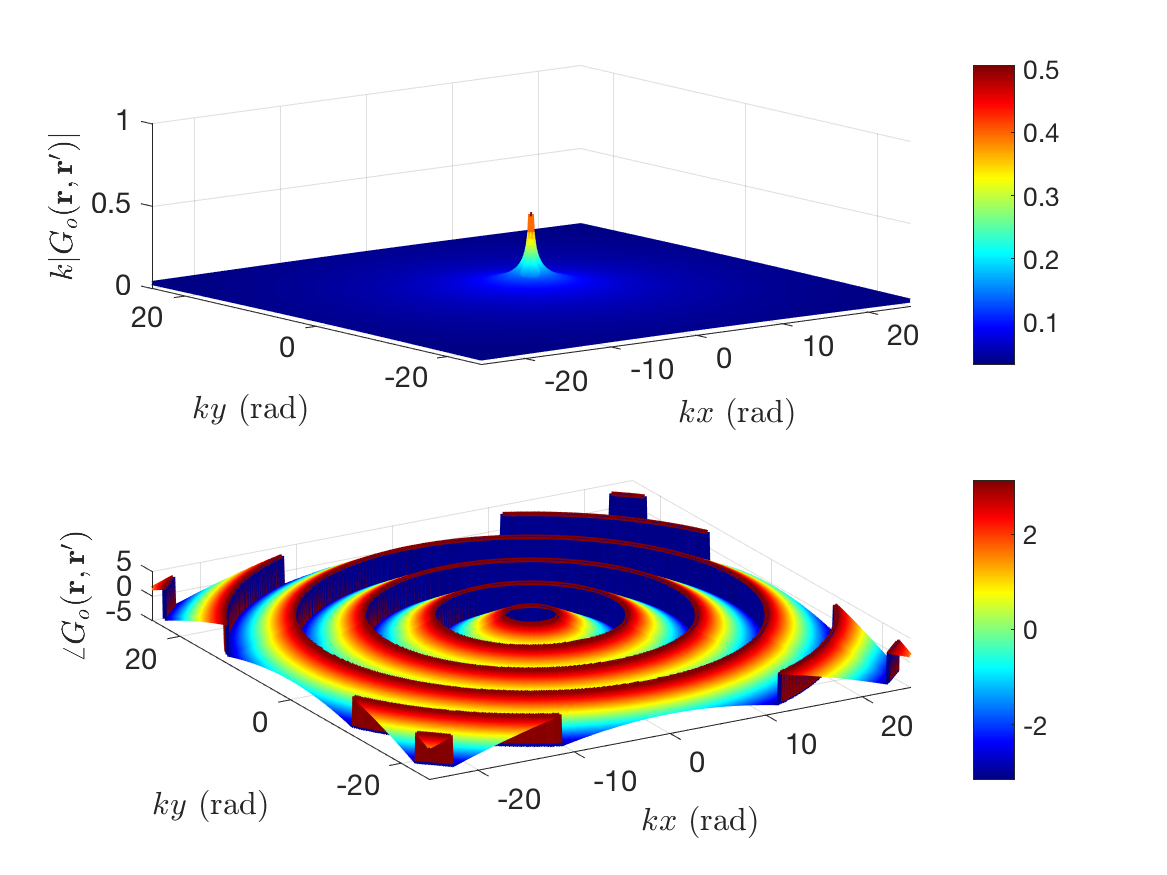
\includegraphics[width=3in]{../media/2d_fs_gf_mag.png}
\end{center}
\renewcommand{\baselinestretch}{1}
\small\normalsize
\begin{quote}
\caption[Magnitude and Phase of 2-D Free Space Green's Function]{Magnitude and Phase of 2-D Free Space Green's Function \label{gf_fig:3}}
\end{quote}
\end{figure} 
\renewcommand{\baselinestretch}{2}
\small\normalsize

\begin{figure}[H]
\begin{center}
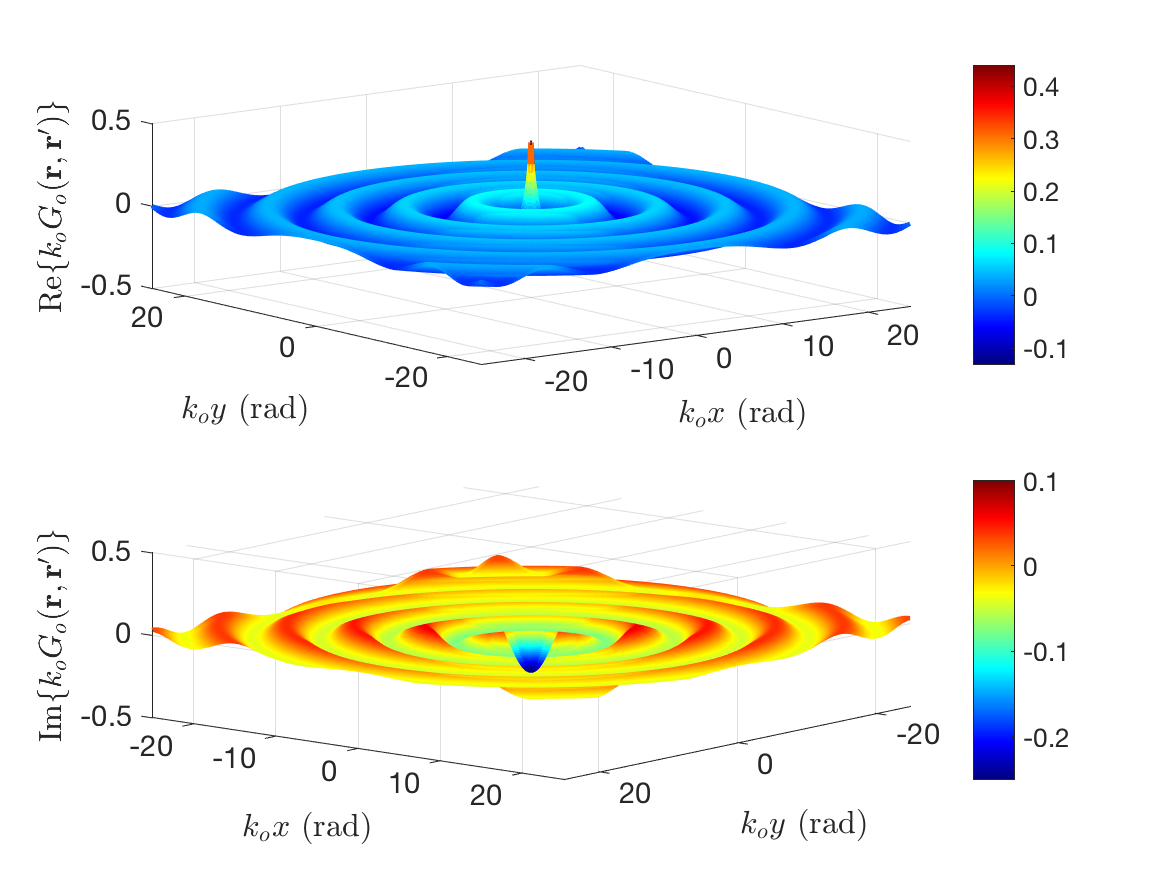
\includegraphics[width=3in]{../media/2d_fs_gf_re_im.png}
\end{center}
\renewcommand{\baselinestretch}{1}
\small\normalsize
\begin{quote}
\caption[Real and Imaginary Components of 2-D Free Space Green's Function]{Real and Imaginary Components of 2-D Free Space Green's Function \label{gf_fig:4}}
\end{quote}
\end{figure} 
\renewcommand{\baselinestretch}{2}
\small\normalsize

\subsubsection{Conversion to the Time Domain}
As in Section \ref{gf_sec:3d}, the Green's function in Equation \ref{gf_eq:40} is still in Fourier space. We can clearly express the frequency dependence as:

\begin{equation}
G_o\left(\boldsymbol{\rho},\boldsymbol{\rho}',\omega\right) = -\frac{j}{4}H_0^{(2)}\left(\frac{\omega}{c}|\boldsymbol{\rho} - \boldsymbol{\rho}' | \right)
\label{gf_eq:40a}
\end{equation}
\renewcommand{\baselinestretch}{2} \small\normalsize

To determine the Green's function in the time domain, we need to take the inverse Fourier transform:
\begin{equation}
\begin{gathered}
G_o\left(\boldsymbol{\rho},\boldsymbol{\rho}',t\right) = \frac{1}{2\pi}\int\limits_{-\infty}^{\infty}d\omega e^{-j\omega t}G_o\left(\boldsymbol{\rho},\boldsymbol{\rho}',\omega\right) \\
G_o\left(\boldsymbol{\rho},\boldsymbol{\rho}',t\right) = -\frac{j}{4}\frac{1}{2\pi}\int\limits_{-\infty}^{\infty}d\omega e^{-j\omega t} H_0^{(2)}\left(\frac{\omega}{c}|\boldsymbol{\rho} - \boldsymbol{\rho}' | \right)\\
\end{gathered}
\label{gf_eq:40b}
\end{equation}
\renewcommand{\baselinestretch}{2} \small\normalsize

We can use a representation of $H_0^{(2)}$ that is related to the Mehler-Sonine integral representation \cite{nist_handbook}:
\begin{equation}
H_o^{(2)}\left(z\right) = -\frac{1}{j\pi}\int\limits_{-\infty}^{\infty}e^{jz\cosh(\tau)}d\tau -\frac{2}{j\pi}\int\limits_{0}^{\infty}e^{jz\cosh(\tau)}d\tau
\label{gf_eq:40c}
\end{equation}
\renewcommand{\baselinestretch}{2} \small\normalsize

\noindent Equation \ref{gf_eq:40c} is valid for $z>0$ . Since $k| \boldsymbol{\rho} - \boldsymbol{\rho}'| > 0$, this condition is satisfied. \\

\noindent Letting $\rho' \rightarrow 0$ for simplification yields:
\begin{equation}
G_o\left(\boldsymbol{\rho},0,t\right) = \frac{1}{4\pi^2}\int\limits_{-\infty}^{\infty}d\omega e^{-j\omega t} \int\limits_{0}^{\infty}e^{j\frac{\omega}{c}\rho\cosh(\tau)}d\tau\\
\label{gf_eq:40d}
\end{equation}
\renewcommand{\baselinestretch}{2} \small\normalsize

\noindent We can bring the integral over $\omega$ inside the integral over $\tau$:
\begin{equation}
\begin{gathered}
G_o\left(\boldsymbol{\rho},0,t\right) = \frac{1}{4\pi^2}\int\limits_{0}^{\infty}d\tau\int\limits_{-\infty}^{\infty}d\omega e^{-j\omega t} e^{j\frac{\omega}{c}\rho\cosh(\tau)}\\
G_o\left(\boldsymbol{\rho},0,t\right) = \frac{1}{4\pi^2}\int\limits_{0}^{\infty}d\tau\int\limits_{-\infty}^{\infty}d\omega e^{-j\omega \left(t - \frac{\rho \cosh(\tau)}{c} \right)}\\
\end{gathered}
\label{gf_eq:40e}
\end{equation}
\renewcommand{\baselinestretch}{2} \small\normalsize

\noindent Again using the definition of the delta function from Equation \ref{gf_eq:30} yields:
\begin{equation}
G_o\left(\boldsymbol{\rho},0,t\right) = \frac{1}{2\pi}\int\limits_{0}^{\infty}d\tau \delta\left(t - \frac{\rho \cosh(\tau)}{c}\right)\\
\label{gf_eq:40f}
\end{equation}
\renewcommand{\baselinestretch}{2} \small\normalsize

For $G_o\left(\boldsymbol{\rho},0,t\right)$ to be nonzero, $t - \frac{\rho \cosh(\tau)}{c} > 0$ for all values of $\tau$. This means $t > \frac{\rho}{c}$ and we can enforce this condition on $t$ through the Heaviside step function, $H\left(t -\frac{\rho}{c}\right)$:
 \begin{equation}
G_o\left(\boldsymbol{\rho},0,t\right) = \frac{1}{2\pi}\int\limits_{0}^{\infty}d\tau H\left(t -\frac{\rho}{c}\right) \delta\left(t - \frac{\rho \cosh(\tau)}{c}\right)
\label{gf_eq:40g}
\end{equation}
 \renewcommand{\baselinestretch}{2} \small\normalsize
 
Because the argument of the delta function is a complicated function of $t$, we need to use the composition property of the delta function \cite{arfken_weber}, \cite{gbur_math}:
 \begin{equation}
\delta\left(g(x) \right) = \sum_{\substack{a \\g(a)=0}}\frac{\delta(x-a)}{|g'(a)|}
\label{gf_eq:40h}
\end{equation}
 \renewcommand{\baselinestretch}{2} \small\normalsize
 
From Equation \ref{gf_eq:40g}, $g(x) = g(\tau) = t - \frac{\rho\cosh(\tau)}{c}$ and the only zero  is $\tau = \cosh^{-1}\left(\frac{ct}{\rho}\right)$. We can now rewrite the delta function from Equation \ref{gf_eq:40g} as:
 \begin{equation}
\delta\left(t - \frac{\rho \cosh(\tau)}{c}\right) = \frac{\delta\left(\tau -\cosh^{-1}\left(\frac{ct}{\rho} \right) \right)}{\rho\sinh\left(\cosh^{-1}\left(\frac{ct}{\rho} \right) \right)}
\label{gf_eq:40i}
\end{equation}
 \renewcommand{\baselinestretch}{2} \small\normalsize
 
\noindent We can now rewrite Equation \ref{gf_eq:40g} as:
 \begin{equation}
 \begin{gathered}
G_o\left(\boldsymbol{\rho},0,t\right) = \frac{1}{2\pi}\int\limits_{0}^{\infty}d\tau H\left(t -\frac{\rho}{c}\right)  \frac{c\delta\left(\tau -\cosh^{-1}\left(\frac{ct}{\rho} \right) \right)}{\rho\sinh\left(\cosh^{-1}\left(\frac{ct}{\rho} \right) \right)}\\
G_o\left(\boldsymbol{\rho},0,t\right) = \frac{cH\left(t -\frac{\rho}{c}\right)}{2\pi \rho\sinh\left(\cosh^{-1}\left(\frac{ct}{\rho} \right) \right)}\int\limits_{0}^{\infty}d\tau \delta\left(\tau -\cosh^{-1}\left(\frac{ct}{\rho} \right) \right)\\
G_o\left(\boldsymbol{\rho},0,t\right) = \frac{cH\left(t -\frac{\rho}{c}\right)}{2\pi \rho\sinh\left(\cosh^{-1}\left(\frac{ct}{\rho} \right) \right)}
\end{gathered}
\label{gf_eq:40j}
\end{equation}
 \renewcommand{\baselinestretch}{2} \small\normalsize
 
\noindent Using the identity that $\sinh\left(\cosh^{-1}(x) \right) = \sqrt{x^2 -1}$:

 \begin{equation}
 \begin{gathered}
G_o\left(\boldsymbol{\rho},0,t\right) = \frac{cH\left(t -\frac{\rho}{c}\right)}{2\pi \rho\sqrt{\left(\frac{ct}{\rho} \right)^2 - 1}     }\\
G_o\left(\boldsymbol{\rho},0,t\right) = \frac{H\left(t -\frac{\rho}{c}\right)}{2\pi \sqrt{t^2 - \left(\frac{\rho}{c}\right)^2}     }
\end{gathered}
\label{gf_eq:40k}
\end{equation}
 \renewcommand{\baselinestretch}{2} \small\normalsize
 
\noindent Letting $t\rightarrow t-t'$ and $\rho \rightarrow \boldsymbol{\rho} - \boldsymbol{\rho}'$ yields the final result:
 \begin{equation}
\boxed{G_o\left(\boldsymbol{\rho},\boldsymbol{\rho}',t,t'\right) = \frac{H\left(t-t' -\frac{|\boldsymbol{\rho} - \boldsymbol{\rho}'|}{c}\right)}{2\pi \sqrt{(t-t')^2 -\left(\frac{|\boldsymbol{\rho} - \boldsymbol{\rho}'|}{c}\right)^2 }     }}
\label{gf_eq:40l}
\end{equation}
\renewcommand{\baselinestretch}{2} \small\normalsize

\subsubsection{Example of Use}
The 2-dimensional free space Green's function is commonly used to describe scattering from wires.


\section{Dyadic Green's Functions}


\section{Stochastic Green's Functions}


